\chapter{Figures}
\label{chap:figures}

Every figure in this chapter is drawn with code, so there are no image files to
manage, and the drawings always match the document's fonts~\cite{tantau2023}.

\begin{tryit}
  Drag an image file from your file manager onto the editor: it is copied into
  \texttt{figures/} and a complete \texttt{figure} environment appears. Copy a
  few cells from a spreadsheet and paste them here: they become a table.
\end{tryit}

\section{Diagrams with TikZ}

\Cref{fig:pipeline} shows what happens inside \rutex{} every time you pause.

\begin{figure}[htbp]
  \centering
  % Diagram in its own file, included with \input from chapters/figures.tex.
\begin{tikzpicture}[
    node distance=6mm and 12mm,
    box/.style={rectangle, rounded corners=3pt, draw=RoyalBlue!70!black, fill=RoyalBlue!10,
                minimum height=9mm, minimum width=24mm, align=center, font=\small, drop shadow},
    tool/.style={box, draw=ForestGreen!70!black, fill=ForestGreen!10},
    arrow/.style={-{Stealth[length=2mm]}, thick, gray!70!black}]
  \node[box] (edit) {You type};
  \node[box, right=of edit] (save) {Autosave\\(atomic)};
  \node[tool, right=of save] (latexmk) {latexmk};
  \node[box, right=of latexmk] (pdf) {PDF viewer\\(Poppler)};
  \node[tool, below=of latexmk] (log) {Log parser};
  \node[box, below=of pdf] (sync) {SyncTeX};
  \draw[arrow] (edit) -- node[above, font=\scriptsize] {pause} (save);
  \draw[arrow] (save) -- (latexmk);
  \draw[arrow] (latexmk) -- (pdf);
  \draw[arrow] (latexmk) -- (log);
  \draw[arrow] (pdf) -- (sync);
  \draw[arrow] (log.west) -| node[below, near start, font=\scriptsize] {error marks} (edit.south);
  \begin{scope}[on background layer]
    \node[fit=(save)(latexmk)(log), draw=gray!40, dashed, rounded corners, inner sep=3mm,
          label={[font=\scriptsize, gray]above:in the background}] {};
  \end{scope}
\end{tikzpicture}

  \caption{The \rutex{} build pipeline.}
  \label{fig:pipeline}
\end{figure}

\begin{figure}[htbp]
  \centering
  \begin{tikzpicture}[
      neuron/.style={circle, draw=RoyalBlue!80!black, fill=RoyalBlue!15, minimum size=7mm, inner sep=0},
      outn/.style={neuron, draw=ForestGreen!80!black, fill=ForestGreen!15},
      x=2.2cm, y=1cm]
    \foreach \i in {1,...,3} \node[neuron] (I\i) at (0,-\i-0.5) {$x_\i$};
    \foreach \i in {1,...,4} \node[neuron] (H\i) at (1,-\i) {};
    \foreach \i in {1,...,2} \node[outn] (O\i) at (2,-\i-1) {$y_\i$};
    \foreach \i in {1,...,3} \foreach \j in {1,...,4} \draw[-{Stealth[length=1.5mm]}, gray] (I\i) -- (H\j);
    \foreach \i in {1,...,4} \foreach \j in {1,...,2} \draw[-{Stealth[length=1.5mm]}, gray] (H\i) -- (O\j);
    \node[above=2mm of I1, font=\small] {input};
    \node[above=2mm of H1, font=\small] {hidden};
    \node[above=2mm of O1, font=\small] {output};
  \end{tikzpicture}
  \caption{A small neural network~\cite{vaswani2017}.}
  \label{fig:network}
\end{figure}

\section{Plots with PGFPlots}

\Cref{fig:plots} combines two plots side by side with \texttt{subcaption}~\cite{feuersanger2021}.

\begin{figure}[htbp]
  \centering
  \begin{subfigure}{0.48\linewidth}
    \centering
    \begin{tikzpicture}
      \begin{axis}[width=\linewidth, height=5.5cm, xlabel={$x$}, ylabel={$y$},
          legend pos=north west, grid=major, grid style={gray!20}]
        \addplot[name path=f, RoyalBlue, thick, domain=0:4, samples=60] {sqrt(x)};
        \addplot[name path=g, BrickRed, thick, domain=0:4, samples=60] {x/2};
        \addplot[RoyalBlue!15] fill between[of=f and g, soft clip={domain=0:4}];
        \legend{$\sqrt{x}$, $x/2$}
      \end{axis}
    \end{tikzpicture}
    \caption{Functions and the area between them.}
  \end{subfigure}\hfill
  \begin{subfigure}{0.48\linewidth}
    \centering
    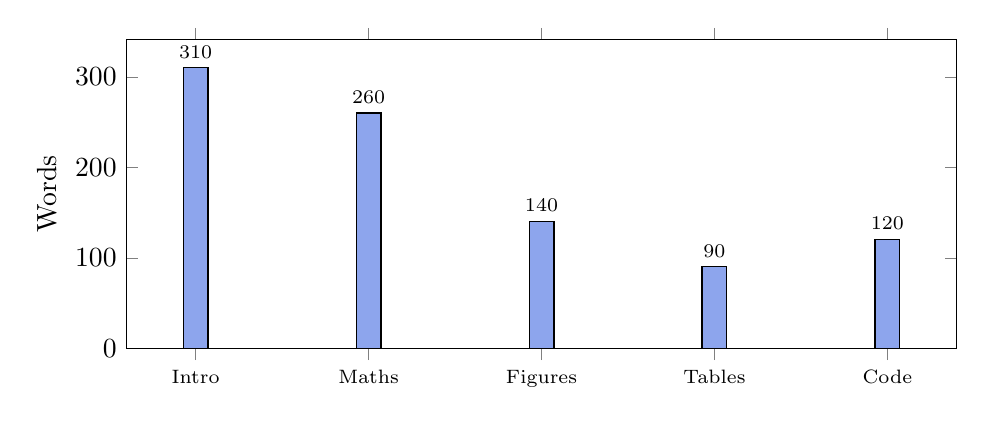
\begin{tikzpicture}
      \begin{axis}[width=\linewidth, height=5.5cm, ybar, bar width=9pt,
          symbolic x coords={Intro, Maths, Figures, Tables, Code}, xtick=data,
          x tick label style={font=\scriptsize}, ylabel={Words}, ymin=0,
          nodes near coords, nodes near coords style={font=\scriptsize}]
        \addplot[fill=RoyalBlue!60] coordinates {(Intro,310) (Maths,260) (Figures,140) (Tables,90) (Code,120)};
      \end{axis}
    \end{tikzpicture}
    \caption{Words per chapter (a bar chart).}
  \end{subfigure}
  \caption{Two plots side by side.}
  \label{fig:plots}
\end{figure}

\begin{figure}[htbp]
  \centering
  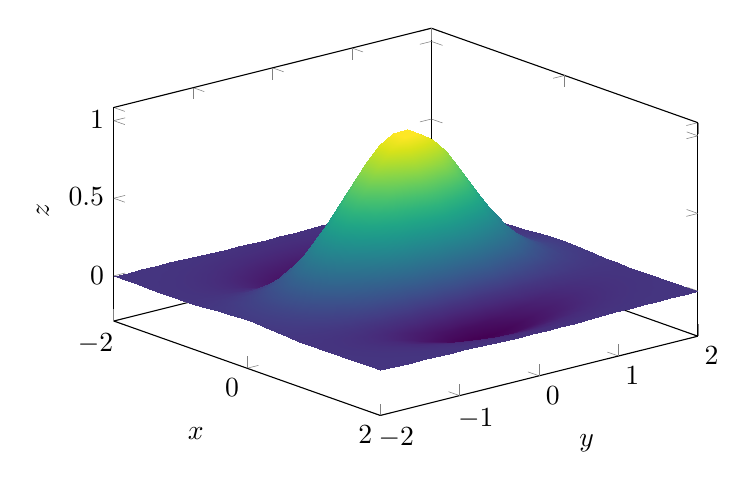
\begin{tikzpicture}
    \begin{axis}[width=9cm, height=6.5cm, view={50}{30}, colormap/viridis,
        xlabel=$x$, ylabel=$y$, zlabel={$z$}]
      \addplot3[surf, domain=-2:2, samples=24, shader=interp] {exp(-x^2-y^2)*cos(deg(2*x))};
    \end{axis}
  \end{tikzpicture}
  \caption{A 3D surface, $z = e^{-x^2-y^2}\cos 2x$.}
  \label{fig:surface}
\end{figure}

\section{Specialised drawings}

\begin{figure}[htbp]
  \centering
  \begin{subfigure}{0.45\linewidth}
    \centering
    \begin{circuitikz}[scale=0.8, transform shape]
      \draw (0,0) to[V, v=$V_s$] (0,3)
            to[R, l=$R_1$] (3,3)
            to[C, l=$C$] (3,0) -- (0,0);
      \draw (3,3) -- (5,3) to[L, l=$L$] (5,0) -- (3,0);
    \end{circuitikz}
    \caption{An RLC circuit (\texttt{circuitikz}).}
  \end{subfigure}\hfill
  \begin{subfigure}{0.45\linewidth}
    \centering
    \begin{forest}
      for tree={draw, rounded corners, fill=RoyalBlue!10, font=\small, s sep=4mm}
      [report
        [preamble]
        [chapters [intro] [maths] [figures]]
        [references]
      ]
    \end{forest}
    \caption{A tree (\texttt{forest}).}
  \end{subfigure}

  \vspace{1em}
  \begin{subfigure}{0.45\linewidth}
    \centering
    \begin{tikzcd}
      A \arrow[r, "f"] \arrow[d, "g"'] & B \arrow[d, "h"] \\
      C \arrow[r, "k"']                & D
    \end{tikzcd}
    \caption{A commutative square (\texttt{tikz-cd}).}
  \end{subfigure}\hfill
  \begin{subfigure}{0.45\linewidth}
    \centering
    \begin{tikzpicture}[->, >={Stealth[length=2mm]}, node distance=17mm, auto,
        every state/.style={fill=RoyalBlue!10, draw=RoyalBlue!70!black, minimum size=9mm, font=\scriptsize}]
      \node[state, initial, initial text=] (idle) {idle};
      \node[state, right=of idle] (build) {build};
      \node[state, accepting, below right=10mm and 4mm of idle] (ok) {ok};
      \path (idle) edge[bend left] node {pause} (build)
            (build) edge[loop above] node {edit} ()
            (build) edge node {done} (ok)
            (ok) edge node {type} (idle);
    \end{tikzpicture}
    \caption{A state machine (TikZ \texttt{automata}).}
  \end{subfigure}
  \caption{Circuits, trees, diagrams and automata.}
  \label{fig:special}
\end{figure}
